\begin{figure}
    \begin{center}
        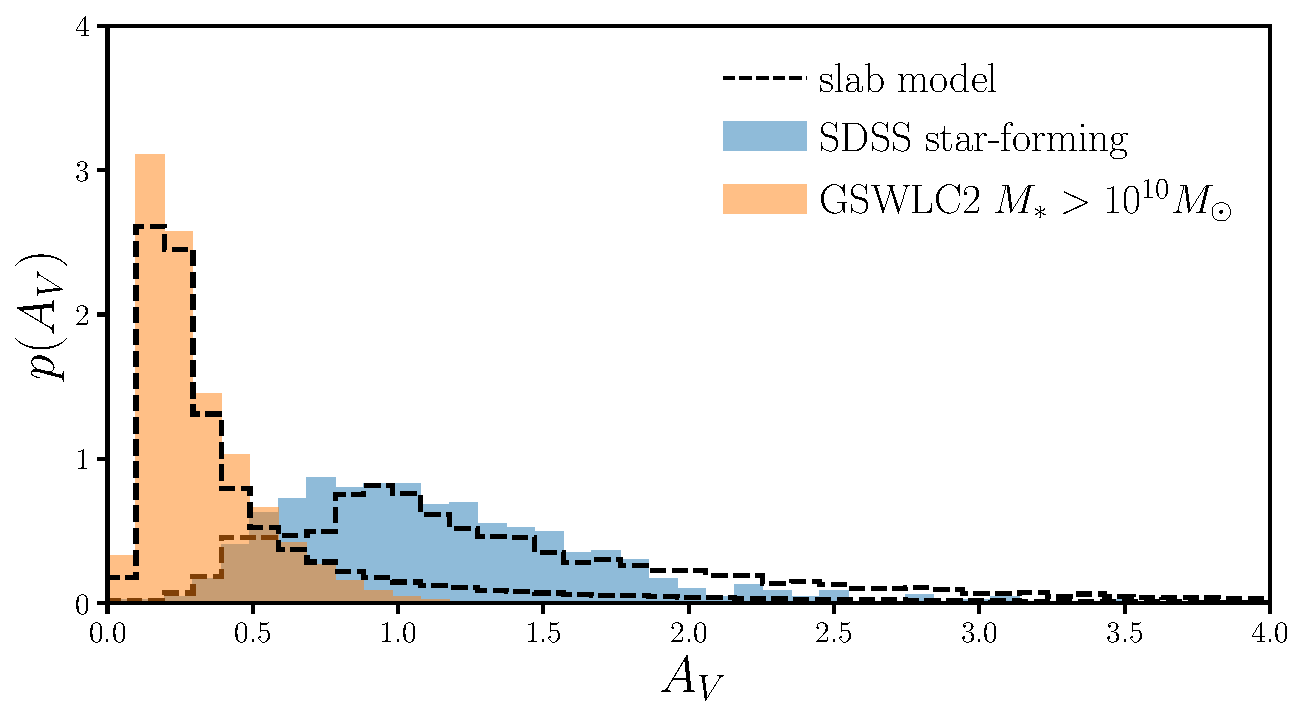
\includegraphics[width=0.66\textwidth]{figs/slab_model.pdf} 
        \caption{\label{fig:av_dist}
        The $A_V$ distributions generated from the slab model (Eq.~\ref{eq:slab};
        black dash) compared to $p(A_V)$ of star-forming galaxies in SDSS
        (blue) and of $M_* > 10^{10}M_\odot$ galaxies in the \cite{salim2018} GSWLC2 sample (orange). 
        The $A_V$ values for both observations are derived using SED
        fitting~\citep{brinchmann2004, salim2018} while the $A_V$ values for
        the slab model are generated using Eq.~\ref{eq:slab} with $M_*$ and
        $\ssfr$ for SDSS and GSWLC2 also measured from SED fitting. 
        The slab model is able to produce $p(A_V)$ in good agreement with
        $p(A_V)$ from both observations. 
        Hence, it provides a sufficiently flexible prescription for our \eda.
        }
    \end{center}
\end{figure}


\section{The Slab Model Based EDA}  \label{sec:slab} 
\ch{ 
    In our \eda~prescription, we use the slab model to determine $A_V$, the
    amplitude of attenuation, as a function of a randomly sampled inclination,
    $i$, and $\tau_V$ (see Eq.~\ref{eq:slab} in Section~\ref{sec:dem}).
    The slab model is based on the assumption that dust in galaxies in
    slab-like geometry and illuminated by the stellar radiation
    source~\citep{somerville1999}. 
}
For a given $\tau_V$, the attenuation depends solely on the orientation of the galaxy. 
\ch{
    While this simplification reproduces the correlation between $A_V$ and $i$
    found in observed star-forming galaxies~\citep[\eg][]{conroy2010, wild2011,
    battisti2017, salim2020}, it ignores the detailed star-to-dust geomtry that
    impacts the attenuation curve. 
    It also does not provide a well-motivated prescription for quiescent
    galaxies, which typically have elliptical morphologies.
    Despite its limitations, the slab model provides a robust empirical
    prescription that allows us to produce realistic distributions of $A_V$. 
}

\ch{ 
    In Figure~\ref{fig:av_dist}, we compare the $A_V$ distributions, $p(A_V)$,
    of star-forming galaxies in SDSS (blue) and galaxies in the
    \cite{salim2018} GSWLC2 sample (orange) to the $p(A_V)$ generated from the
    slab model (black dashed). 
    The $A_V$ values of the SDSS are derived using SED fitting from the
    \cite{brinchmann2004} MPA-JHU catalog.
    The $A_V$ values of the GSWLC2 galaxies are also derived from SED fitting UV and optical
    photometry from GALEX and SDSS observations as well as mid-IR photometry from WISE. 
    We include all GSWLC2 galaxies, including quiescent galaxies, above $M_* > 10^{10}M_\odot$. 
    We include slab model $A_V$ distributions for SDSS and GSWLC2 individually.
    We sample $A_V$ for each SDSS and GSWLC2 galaxy: we uniformly sample $\cos
    i$ from 0 to 1 and derive $\tau_V$ (Eq.~\ref{eq:tauv}) with $M_*$ and
    $\ssfr$ measured from SED fitting. 
    We pick $\mtaum, \mtaus, c_\tau$ values within the prior range
    (Table~\ref{tab:free_param}) to reproduce the SDSS and GSWLC2 $p(A_V)$
    distirbutions by eye. 
    The comparison reveals that the slab model can produce $p(A_V)$ in good
    agreement with both observed distributions. 
    We therefore conclude that the slab model provides a sufficiently flexible
    prescription to sample a realistic distribution of $A_V$. 
}


\ch{
    In addition to assuming the slab model, in the \eda, we also assume 
    a linear dependence on $M_*$ and $\ssfr$ in the $V$ band optical depth,
    $\tau_V$ (see Eq.~\ref{eq:tauv}).
    This parameterization is motivated by observations that find significant
    correlation between $A_V$ and $M_*$ and $\ssfr$~\citep[\eg~][]{garn2010, battisti2016, salim2020}. 
    We take a closer look at this correlation using the GWSLC2 sample in
    Figure~\ref{fig:dep}.
    We present the dependence of $A_V$ on $M_*$ (left panel) and $\ssfr$ (right
    panel). 
    In the left panel, we divide the GSWLC2 galaxies by $\ssfr$: 
    $-11 < \log \ssfr < -10.5$ (purple),  $-10.5 < \log \ssfr < -10$ (red),
    and  $-10 < \log \ssfr$ (orange). 
    For each of the $\ssfr$ bins, we find significant $\log M_*$ dependence in
    $A_V$. 
    Galaxies with higher $\ssfr$ have a stronger $M_*$ dependence.  
    In the right, we divide the galaxies by $M_*$: 
    $9.5 < \log M_* < 10.5$ (blue) and $10.5 < \log M_* < 11.5$ (green).
    Although both $M_*$ bins have some $\ssfr$ dependence, the dependence is
    stronger for galaxies with $M_* > 10^{10.5}M_\odot$. 
    This stellar mass limit roughly corresponds to galaxies that are included
    in our forward model (see Figure~\ref{fig:avmsfr}). 
    The $M_*$ and $\ssfr$ dependence we find in $A_V$ from the GSWLC2 sample is
    consistent with previous observations.
    Moreover, the $M_*$ and $\ssfr$ dependence we find further motivates our
    \eda~prescription.
}

\begin{figure}
\begin{center}
    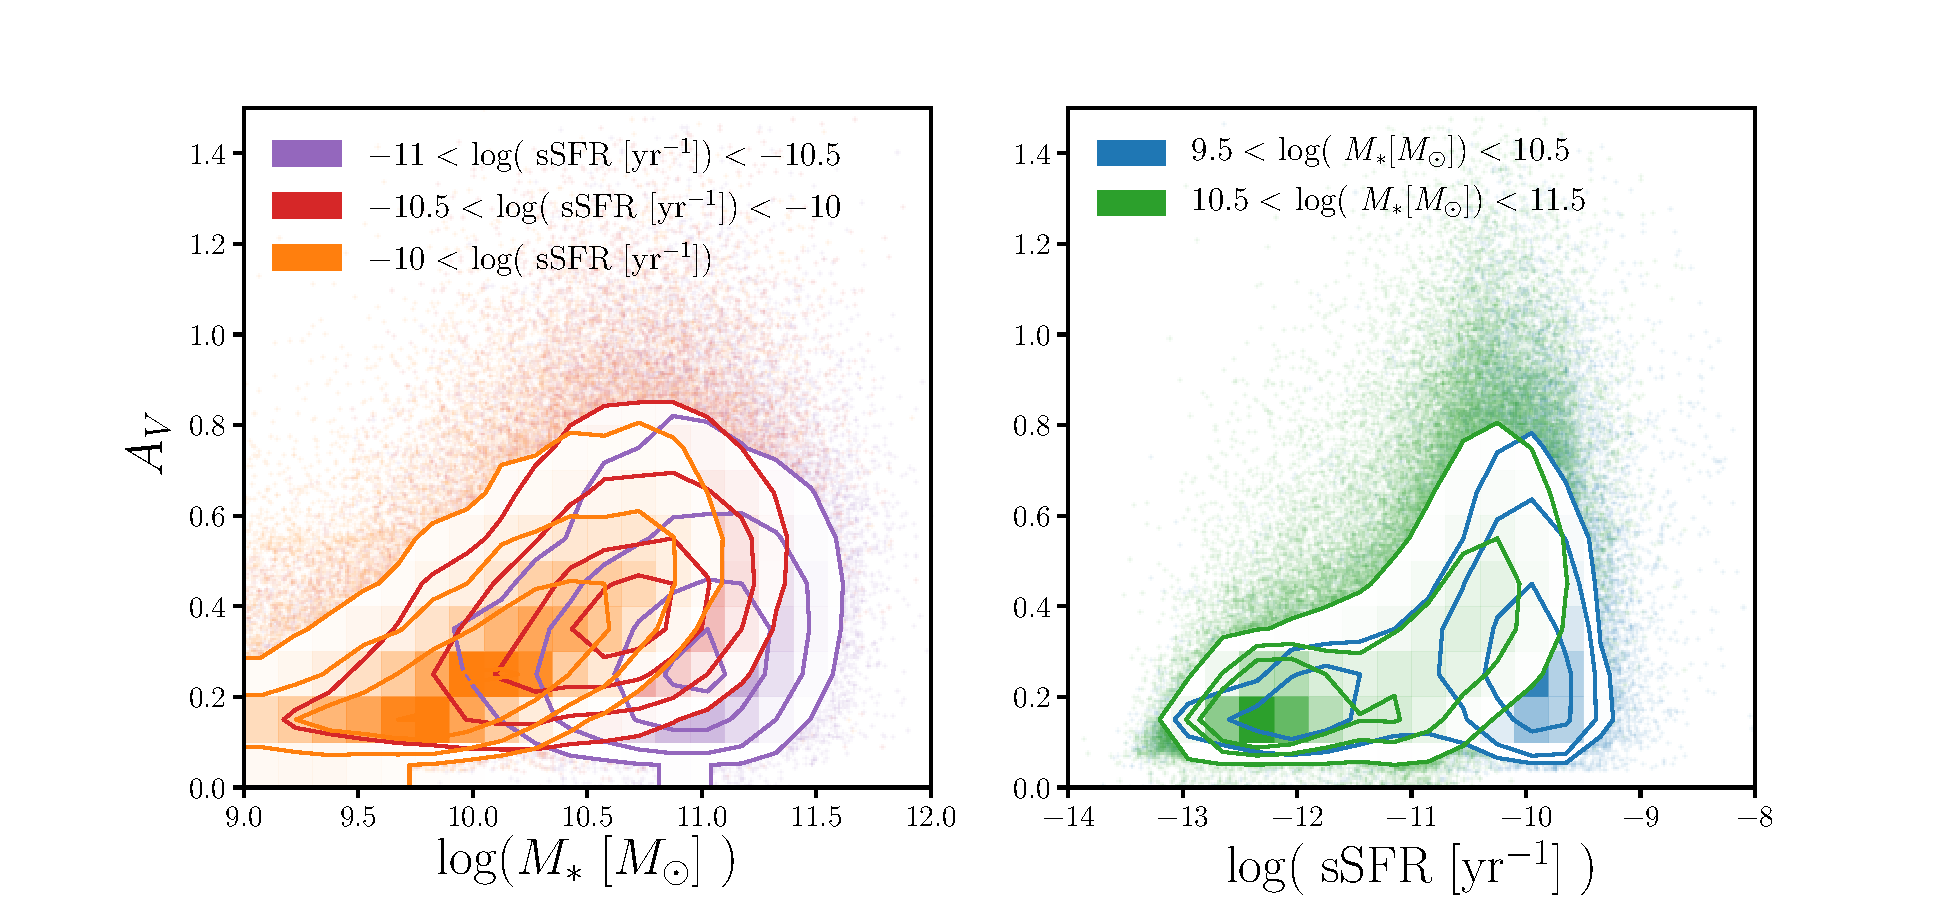
\includegraphics[width=\textwidth]{figs/gswlc_Av_mstar_ssfr_dependence.pdf}
    \caption{\label{fig:dep}
    \ch{
        Dependence of $A_V$ on  $M_*$ (left) and $\ssfr$ (right) for the
        \cite{salim2018} GSWLC2 sample.
        In the left panel, we divide the GSWLC2 sample into bins of $\ssfr$: 
        $-11 < \log \ssfr < -10.5$ (purple),  $-10.5 < \log \ssfr < -10$ (red),
        and  $-10 < \log \ssfr$ (orange). 
        There is a significant $M_*$ dependence in all of the $\ssfr $bins. 
        In the right panel, we divide the sample into bins of $M_*$:  
        $9.5 < \log M_* < 10.5$ (blue) and $10.5 < \log M_* < 11.5$ (green).
        In the $\log M_* > 10.5$ bin, which roughly corresponds to our SDSS
        sample, we find significant $\ssfr$ dependence.
        The $M_*$ and $\ssfr$ dependence in $A_V$ we find in GSWLC2, which is
        consistent with previous observations, provides further motivation for 
        our \eda~prescription.
    }
    }
\end{center}
\end{figure}
